\documentclass[10pt]{beamer}

\usetheme[progressbar=frametitle]{metropolis}
\usepackage{appendixnumberbeamer}
\usepackage[utf8]{inputenc}
\usepackage{booktabs}
\usepackage[scale=2]{ccicons}
\usepackage{xcolor}
\usepackage{pgfplots}
\usepgfplotslibrary{dateplot}
\usepackage{xspace}


\usepackage{listings}


% Emulate markdown's light grey background for monospace.
\usepackage{soul}
\definecolor{Light}{gray}{.96}
\sethlcolor{Light}
\let\OldTexttt\texttt
\renewcommand{\texttt}[1]{\OldTexttt{\hl{#1}}}% will affect all \texttt


%  Use knitr's colorscheme.
\definecolor{fgcolor}{rgb}{0.345, 0.345, 0.345}
\definecolor{hlnum}{rgb}{0.686,0.059,0.569}
\definecolor{hlstr}{rgb}{0.192,0.494,0.8}
\definecolor{hlcom}{rgb}{0.678,0.584,0.686}
\definecolor{hlopt}{rgb}{0,0,0}
\definecolor{hlstd}{rgb}{0.345,0.345,0.345}
\definecolor{hlkwa}{rgb}{0.161,0.373,0.58}
\definecolor{hlkwb}{rgb}{0.69,0.353,0.396}
\definecolor{hlkwc}{rgb}{0.333,0.667,0.333}
\definecolor{hlkwd}{rgb}{0.737,0.353,0.396}
\definecolor{shadecolor}{rgb}{0.969, 0.969, 0.969}

\lstset{
  backgroundcolor=\color{shadecolor},
  basicstyle=\color{hlstd}\sffamily\footnotesize,
  breakatwhitespace=false,
  %breaklines=true,
  captionpos=b,
  commentstyle=\color{hlcom},
  deletekeywords={...},
  escapeinside={\%*}{*)},
  extendedchars=true,
  frame=lines,
  keepspaces=true,
  keywordstyle=\color{hlkwb},
  morekeywords={*,...},
  numbers=left,
  numbersep=5pt,
  numberstyle=\tiny\color{hlstd},
  rulecolor=\color{hlstd},
  showspaces=false,
  showstringspaces=false,
  showtabs=false,
  stepnumber=1,
  stringstyle=\color{hlstr},
  tabsize=2,
  title=\lstname
}

\newcommand{\themename}{\textbf{\textsc{metropolis}}\xspace}

\title{KodeKlubben 2.0}
\subtitle{Øvelsesgang 2}
% \date{\today}
\date{\today}
\author{Kristian Urup Olesen Larsen, Jakob Jul Elben}
\institute{Økonomisk Institut, KU}
% \titlegraphic{\hfill\includegraphics[height=1.5cm]{logo.pdf}}

\begin{document}

\maketitle

\begin{frame}[fragile]{Velkommen (igen)!}
Hvem er vi?
\begin{itemize}
  \item Økonomistuderende
  \item RA's på Økonomisk Institut
  \item Arbejder typisk i Python, R, STATA eller SAS
\end{itemize}
Hvem er i?
% \begin{itemize}
%   \item Det er sådan set ligemeget, vi skal bare have det sjovt og lære noget \textit{data science}.
% \end{itemize}
\end{frame}

\begin{frame}[fragile]{Setup}
  Alt materiale ligger på GitHub
\begin{itemize}
  \item Åben \href{https://github.com/Kristianuruplarsen/kodeklubben}{https://github.com/Kristianuruplarsen/kodeklubben}
  \item Klik på knappen \textit{Clone or download} og på \textit{Download ZIP}
\end{itemize}

\begin{figure}
  \center
  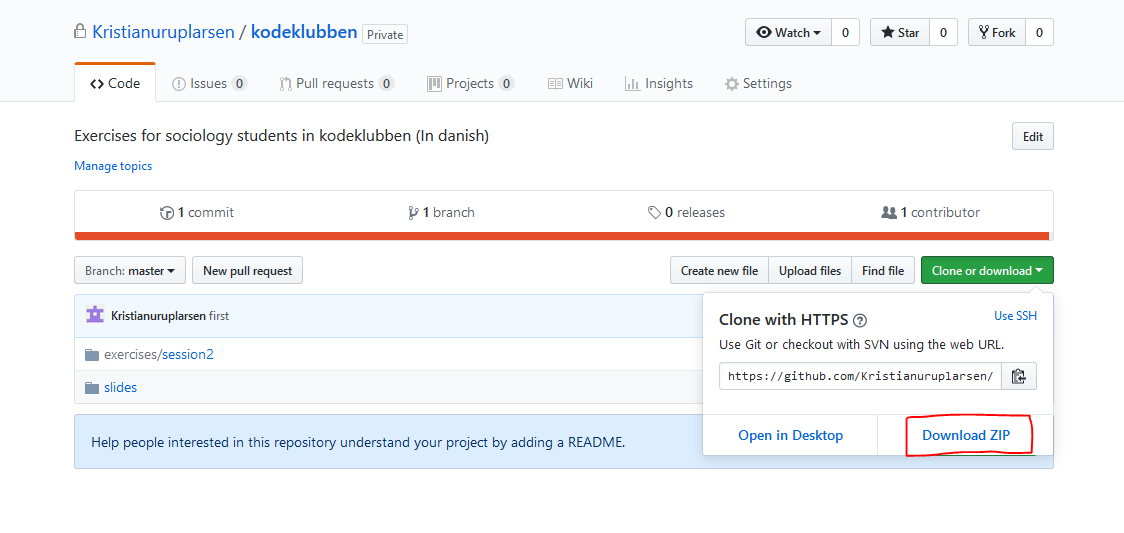
\includegraphics[width=\textwidth]{figs/setup.PNG}
\end{figure}
\end{frame}

\begin{frame}[fragile]{Sidste gang}
Sidste gang downloadede og rensede vi et datasæt over danske kommunalpolitikeres holdninger:
\begin{itemize}
  \item Åben det datasæt i selv gemte sidste gang, eller
  \item Hent datasættet online:
  \begin{lstlisting}[language=python]
import pandas as pd

url = 'https://raw.githubusercontent.com/'\
      'Kristianuruplarsen/kodeklubben/master/'\
      'data/candidates.csv'
df = pd.read_csv(url)
  \end{lstlisting}
\end{itemize}
\end{frame}

\begin{frame}[fragile]{Projektet}
\textcolor{gray}{Sidste gang:}
\begin{itemize}
  \item[\textcolor{gray}{$\bullet$}] \textcolor{gray}{Download data fra DR}
  \begin{itemize}
    \item[\textcolor{gray}{$\bullet$}] \textcolor{gray}{internet-hacks}
    \item[\textcolor{gray}{$\bullet$}] \textcolor{gray}{Interagere med nettet gennem python}
  \end{itemize}
  \item[\textcolor{gray}{$\bullet$}] \textcolor{gray}{Rens datasættet og gør klar til alt det sjove}
  \begin{itemize}
    \item[\textcolor{gray}{$\bullet$}] \textcolor{gray}{jonglere med data og formatter}
  \end{itemize}
\end{itemize}

Denne gang:
\begin{itemize}
  \item Alt det sjove.
  \begin{itemize}
    \item \textit{Dimensionality reduction}
    \item Interaktive plot
  \end{itemize}
\end{itemize}
\end{frame}





\section{Øvelser}

\begin{frame}[fragile]{Structure data}
Load data, enten dem i gemte sidste gang, eller fra github (brug koden fra slides)
 \textit{Hint:} denne gang skal i bruge pakken \texttt{pandas} (installer den med pip hvis i ikke allerede har den) som er pythons dataset-workhorse. Som regel kan man google sig til en løsning med søgeord a-la "pandas load dataset from github", "pandas convert to string" osv.
\end{frame}

\begin{frame}[fragile]{Structure data}
Dette gøres ved
  \begin{lstlisting}[language=python]
import pandas as pd

url = 'https://raw.githubusercontent.com/'\
      'Kristianuruplarsen/kodeklubben/master'\
      '/data/candidates.csv'

df_raw = pd.read_csv(url)
\end{lstlisting}
\end{frame}

\begin{frame}[fragile]{Structure data}
Lige nu er kandidaternes svar registreret i en enkelt streng af tal mellem 1 og 5. Et 1-tal svarer til at kandidaten har svaret det mest venstrestille ("Meget uenig"), 5 svarer ligeledes til det meste højrestillede ("Meget enig").

Konverter kolonnen 'answers' til en streng-variable og drop de kandidater der ikke har svaret på alle spørgsmålene fra datasættet. Hvor mange observationer mister i?

Skriv dernæst en funktion der spreder answerstring ud over 15 variable (hint: stackoverflow).
\end{frame}


\begin{frame}[fragile]{Structure data}
Dette gøres ved
  \begin{lstlisting}[language=python]
df = df_raw

df['answers'] = df['answers'].astype(str)   # convert to string
df['Ncomplete'] = df.answers.apply(len)     # find no.
                                            # answered questions
df = df.query("Ncomplete == 15").reset_index(drop = True)
            # remove if less than 15 answers are answered

df = pd.concat([df, df['answers'].
    apply(lambda x: pd.Series(list(x)))], axis = 1)

df
\end{lstlisting}
\end{frame}

\begin{frame}[fragile]{PCA}
Nu har i et pænt, færdigt datasæt. Næste step er at lave den interaktive figur i så til at starte med sidste fredag. For at lave den skal vi igennem et par trin:

  \begin{itemize}
    \item  Vi skal have kollapset svarende på de 15 spørgsmål til tre akser - til det bruger vi PCA
    \item  Vi skal have skrevet noget kode der producerer interaktive figurer, i får noget af koden udleveret her, fordi det kræver en hel del ligegyldig kode at sætte op.
  \end{itemize}
\end{frame}

\begin{frame}[fragile]{PCA}
Opgave 2.1 - PCA (≈machine learning)

Ligesom at pandas er pythons workhorse for datasæt, er scikit-learn goto pakken for machine learning i python. Start med at installere scikit learn. Læs derefter lidt af denne guide til PCA modulet. Forsøg at få et overblik over

  \begin{itemize}
    \item Hvordan man importerer PCA modulet, og hvordan man bruger det
    \item  Hvordan PCA virker - hvad er idéen bag algoritmen?
  \end{itemize}

Estimer en PCA model med 3 komponenter på de 15 kolonner med politikernes svar, jeres output skal have tre kolonner og lige så mange rækker som i har observationer i datasættet.
\end{frame}
\end{document}
